% declare our document type
\documentclass[12pt]{article}

%%%%%%%% PACKAGES NEEDED FOR THIS DOCUMENT

% allow us to put pictures in the document
\usepackage{graphicx}
% this line lets us use larger fonts
\usepackage{extsizes}
% this allows us to create ''slides'' in the document
\usepackage[most]{tcolorbox}
% this line lets us caption images inside the ''slides''
% this is neccesary since the slide doesn't allow the use of
% \figure{} inside
\usepackage{caption}
\usepackage{courier}
\usepackage[hidelinks]{hyperref}
\usepackage[margin=1in]{geometry}
\usepackage[utf8]{inputenc}
\usepackage[english]{babel}
\usepackage{cite}
\usepackage{listings}
\usepackage{textcomp}

\usepackage[T1]{fontenc}


%%%%%%%%%%% CUSTOM ENVIRONMENT SETUP

% declare a typesetting environment for code/emphasis
\newcommand{\code}[1]{\texttt{\bfseries#1}}
\newenvironment{codeblock}{\bfseries\texttt\bgroup}{\egroup\par}
% declare a large font environment for use in the ''slides''
\newcommand{\instruction}[1]{\Large{#1}}
\newenvironment{instructionblock}{\Large\bgroup}{\egroup}
% declare a ''slide'' text box for use in the document
% the slide is a numbered \section{}
\newtcolorbox[auto counter]{slide}[3][]{%
colback=brown!5!white,colframe=brown!80!gray,height=3.72in,
title={\addcontentsline{toc}{section}{\thetcbcounter ~~ #2}\bf\Large\thetcbcounter ~ #2\hfill #3 \label{slide \thetcbcounter}\setcounter{section}{\thetcbcounter}}}
% declare a ''subslide'' text box for use in the document
% the subslide is a numbered \subsection{}
\newtcolorbox[auto counter,number within=section]{subslide}[3][]{%
colback=blue!5!white,colframe=blue!80!gray,height=3.72in,
title={\addcontentsline{toc}{subsection}{\thetcbcounter ~~ #2}\bf\Large\thetcbcounter ~ #2\hfill #3 \label{slide \thetcbcounter}}}
\renewcommand{\labelitemii}{$\circ$}
\lstset{basicstyle=\ttfamily,keywordstyle=\bfseries\color{blue!80!black},identifierstyle=\bfseries,stringstyle=\color{red},showstringspaces=false,commentstyle=\itshape\color{green!40!black},upquote=true}

% My Environments (keep these)
\newcommand{\ben}{\begin{enumerate}}
\newcommand{\een}{\end{enumerate}}
\newcommand{\bi}{\begin{itemize}}
\newcommand{\ei}{\end{itemize}}
\usepackage{titling}% for changelog
\newcounter{questionEnumerate}
\usepackage[anythingbreaks]{breakurl}%for breaking long url in references

%%%%%%%%% SET UP OUR TITLE PAGE

\begin{document}
\title{ Network Scanning \\ \large  NMap and NetCat}
\author{Venkata SreeKrishna K. and Lavanya K. Galla \\ Revisions added by Hannah Pearson and Dillon Harris}
\date{July 8, 2017 \\ \hyperref[changelog]{Version 4.1}} %\today
\renewcommand{\abstractname}{Executive Summary}
\begin{titlepage}
\maketitle
\keepthetitle % for changelog
\pagenumbering{gobble}
\begin{center}

\includegraphics[scale=.5]{UofI}

\large{CS 539: Applied Security Concepts}

\vskip 40pt

\end{center}
\begin{abstract}
NMap is a port scanning tool that can be used to detect hosts and services running on a particular network. Identifying hosts on a network is important because you can determine whether services with known vulnerabilities are already running and decide what attack vectors are most likely to be successful. In this tutorial, basic NMap functions are demonstrated and some more advanced features are mentioned. For the first part of this tutorial, you will be scanning a specified IP range and creating a network map. 

NetCat is used to transfer data over a network using TCP or UDP. It was designed to be a reliable back-end tool that can be used by other programs and scripts. Like NMap, NetCat can be used for port scanning. However, it is more commonly used for sending data over a network. More relevant to our purposes, NetCat can be used to set up a reverse shell on a target computer and establish persistence. In this tutorial, we will use NetCat to create a chat program as well as to acquire remote shells.

\center{\textbf{Prerequisites}}

Basic knowledge of networking, ports, and the bash command line.
\end{abstract}


\vfill
\begin{center}
	
\includegraphics[scale=0.5]{cc}
	\vskip 10pt
	This work is licensed under a \href{https://creativecommons.org/licenses/by/4.0/}{Creative Commons Attribution 4.0 International License}.
\end{center}

\end{titlepage}

%%%%%%%%%% TABLE OF CONTENTS

\pagebreak
\tableofcontents

%%%%%%%%%%%%%%%%%%%%%%%%%%%%%%%%%%%%%%%%%%%%%%%%%
%%%%%%    BEGINNING OF ACTUAL DOCUMENT
%%%%%%%%%%%%%%%%%%%%%%%%%%%%%%%%%%%%%%%%%%%%%%%%%

\pagebreak
\pagenumbering{arabic}
\setcounter{section}{1}
\begin{slide}{ NMap Overview}{\hyperref[slide 2]{\textgreater}}
   \vskip 10 pt
   \begin{instructionblock}
      \begin{itemize}
         \item NMap: 
            \bi
            \item Port scanning tool; 
            \item Used for network mapping and host discovery;
            \item First released on September 1, 1997;
            \item Free and open source;
            \item Designed to rapidly scan large networks;
            \item Graphical interface Zenmap is available;
            \item Supports Unix and variants, Windows, and Mac OS.
            \ei
      \end{itemize}
   \end{instructionblock}
\end{slide}
NMap is a free software (GPLv2) network and port scanner. It is a command line tool that can identify hosts on a network, classify the status of ports on known hosts, and speculate what the operating system of a scanned host is \cite{NMap}. 

The primary legitimate task it is used for is keeping track of network resources and uptime. However, it can be illegitimately used to scan someone else's network to identify vulnerabilities. For this reason, it is never a good idea to scan a network unless you have written permission from the appropriate authority. 

Using NMap to scan a network without such permission strays into various levels of illegality, depending on the jurisdiction you reside in. It could get you sued or maybe even imprisoned. It goes without saying that it's good practice to always double-check the address you are about to scan with NMap.

NMap is useful because it has a massive variety of arguments that can be passed to it, can scan entire networks very quickly, is built for every major operating system (and in some cases can come packaged with a GUI), and can even be used to scan the ports of local host.

\pagebreak
\begin{slide}{Features}{\hyperref[slide 1]{\textless}\hyperref[slide 3]{\textgreater}}
   %\vskip 10 pt
   \begin{instructionblock}
      \begin{enumerate}
         \item Port Scanning; 
         \item Operating System Detection;
         \item Version Detection;
         \item Host Discovery;
         \item Scripting Interaction.
      \end{enumerate}
   \end{instructionblock}
\end{slide}
%\vfill
\begin{enumerate}
   \item 

Port scanning is used to create a list of all the open ports on target hosts. In general port scan is a process that sends client request to a range of server port addresses on a host with a goal of finding an active port.

\item One of NMap's best-known features is remote OS detection using TCP/IP stack fingerprinting. NMap sends a series of TCP and UDP packets to the remote host and examines practically every bit in the responses. If NMap is unable to guess the OS of a machine, and conditions are good,  NMap will provide a URL you can use to submit the fingerprint if you know (for sure) the OS running on the machine. 
\cite{book} 

\item Using its NMap-services database of about 2,200 well-known services,  NMap would report that those ports probably correspond to a mail server (SMTP), web server (HTTP), and name server (DNS) respectively. This lookup is usually accurate—the vast majority of daemons listening on TCP port 25 are, in fact, mail servers.

\item Host discovery is a service which is used to identify hosts on a network. For example, listing the hosts that respond to TCP or ICMP request or have a particular port open.

\item NMap scripting Engine allows users to write and share simple scripts using the Lua programming language  to automate a wide variety of networking tasks.
\cite{book} 
\end{enumerate}
\pagebreak
\begin{slide}{Legal Issues}{\hyperref[slide 2]{\textless}\hyperref[slide 4]{\textgreater}}
   \vskip 10 pt
   \begin{instructionblock}
      \begin{itemize}
         \item Unauthorized port scanning is illegal;
         \item Do not scan networks without permission;
         \item Reconnaissance can be interpreted as malicious intent;
            \item Summary: Check your address ranges before scanning.
      \end{itemize}
   \end{instructionblock}
\end{slide}
%\vfill

There are legal issues associated with using NMap to scan a computer, network, or domain where you do not have explicit authorization to do so. In many jurisdictions, using NMap to scan a random website or computer is illegal or leaves you with the possibility of getting sued or your internet service provider revoking your internet service.
\cite{ NMap} 

\pagebreak

%\begin{slide}{Related News}{\hyperref[slide 3]{\textless}\hyperref[slide 5]{\textgreater}}
%  \vskip 10 pt
%  \begin{instructionblock}
%     \begin{enumerate}
%        \item Latest version NMap 7 has faster scanning and improved IPv6 support\cite{nmap7}
%        \item SourceForge accused of hijacking NMap project account\cite{sourceforge}
%     \end{enumerate}
%  \end{instructionblock}
%\end{slide}
%\vfill
%\begin{enumerate}

%\item Version 7 of NMap moved a lot of code written in old, unsustainable C into the  NMap Scripting Engine (NSE), which has scripts written in Lua. This means that a lot of  NMap functionality is now coded into the NSE, where it is easier to maintain and modify for special purposes.  NMap 7 brings more IPv6 and SSL\slash TLS support. Also, it scans faster.\cite{nmap7}

%\item The developer of NMap, Gordon "Fyodor" Lyon, accused SourceForge of restricting his access to the  NMap code and installers hosted on the SourceForge website. He said that SourceForge moved the content to a new page that he has no control over. In the past, SourceForge has been caught committing other unethical acts in regards to free software, such as bundling adware with old versions of GIMP available for download from their website.\cite{sourceforge}

%s\end{enumerate}

\pagebreak
\begin{slide}{ NMap: Introduction}{\hyperref[slide 3]{\textless}\hyperref[slide 5]{\textgreater}}
   %\vskip 10 pt
   \begin{instructionblock}
 Several options for port scans:
         \bi
         \item DNS lookup;
         \item Ping scans (check if hosts are up and not filtered);
         \item Different packet types;
         \item Firewall evasion.
         \ei
 NMap scan results include a list of ports and the state of each port, which is one of the following: open, closed, filtered, unfiltered, open|filtered, closed|filtered.
\end{instructionblock}
\end{slide}
%\vfill

Initially when an IP address is selected for scanning,  NMap looks up the DNS server and resolves the IP. Then  NMap pings each of the ports by sending a zero byte packet. If the packets are not received back then it means that the port is closed and if the packets are received back then the port is said to be open.  NMap then sends different packets with different timing to determine whether the port is filtered or unfiltered. If firewalls are present on those systems they can interfere with the process.\\

%\pagebreak
%\begin{slide}{ NMap Port States}{\hyperref[slide 5]{\textless}\hyperref[slide 7]{\textgreater}}
%  \begin{instructionblock}
%     \begin{enumerate}
%        \item Open - a service is running on the port
%        \item Closed - port responds, but no service is running
%        \item Filtered - meaning it is protected
%        \item Unfiltered - unable to determine port status
%        \item Open | Filtered - indeterminate between these states
%        \item Closed | Filtered - indeterminate
%     \end{enumerate}
%  \end{instructionblock}
%\end{slide}
%\vfill

Here is a more detailed explanation of port states:
\begin{enumerate}
   \item An open port actively responds to an incoming connection. It shows the available services on the port. \cite{cookbook} 
   \item A closed port is a port on a target that actively responds to a probe but does not have any service running on the port. Closed ports are commonly found on systems where no firewall is in place to filter incoming traffic.\cite{cookbook} 
   \item Filtered ports are those which are typically protected by a firewall of some sort that prevents  NMap from determining whether or not the port is open or closed.\cite{cookbook} 
   \item An unfiltered port is a port that  NMap can access but is unable to determine whether it is open or closed.\cite{cookbook} 
   \item An open|filtered port is a port which  NMap believes to be open or filtered but cannot determine which exact state the port is actually in.\cite{cookbook} 
   \item A closed|filtered port is a port that  NMap believes to be closed or filtered but cannot determine which respective state the port is actually in.\cite{cookbook} 
\end{enumerate}

\pagebreak
\begin{slide}{ NMap: Target Specification}{\hyperref[slide 4]{\textless}\hyperref[slide 6]{\textgreater}}
   %\vskip 10 pt
   \begin{instructionblock}
General syntax: \code{nmap [target(s)]}. \\ Examples of specific options that can be used:
      \begin{itemize}
\item One IPv4 address: \code{nmap 192.168.0.1};
\item A range of IPv4 addresses: \code{nmap 192.168.0.1-100};
\item A subnet: \code{nmap 192.168.0.0/24};
\item Excluding specific IPs: \code{nmap 192.168.0.0/24 --exclude 192.168.0.1}.
      \end{itemize}
   \end{instructionblock}
\end{slide}

Executing  NMap with no command line options will perform a basic scan on the specified target. A target can be specified by IP address or host name. A default  NMap scan will check for the 1000 most commonly used TCP/IP ports \cite{cookbook}. 
\\ \\
Note that while  NMap can be used to scan IPv6 targets, using the \code{-6} option, some features such as scanning multiple targets using ranges are not supported \cite{cookbook}.\\
Example: \code{\$ nmap -6 fe80::29aa:9db9:4164:d80e}
\\ \\

\pagebreak
\begin{slide}{NMap: Task 1}{\hyperref[slide 5]{\textless}\hyperref[slide 7]{\textgreater}}
   %\vskip 10 pt
   \begin{instructionblock}
    \textbf{Task 1:} Scan the network you are on now. There are several machines on this network located in a hidden folder. Write down the ip addresses of any hosts you find.
   \end{instructionblock}
\end{slide}

Hint: Look at previous slide for syntax help. If that is inadequate, man nmap is always a good option. Third resort: quietly shout at your neighbor or me or someone else and we'll help.



\pagebreak
\begin{slide}{ NMap: Commonly Used Options}{\hyperref[slide 6]{\textless}\hyperref[slide 8]{\textgreater}}
   %\vskip 10 pt
   \begin{instructionblock}
      \begin{enumerate}
\item Aggressive Scan: \code{nmap -A [target]};
\item OS detection: \code{nmap -O [target]};
\item Write output to xml file: \code{-oX [filename]}.
      \end{enumerate}
\textbf{Task 2:} Scan the network again and save the output to an XML file.

\vspace{16mm}
Try using different options and note the difference in scan time and results.
   \end{instructionblock}
\end{slide}
%\vfill
Note that, as common for command line utilities, it is possible to specify multiple options at once.\\

The -A specifies an aggressive scan. The aggressive scan selects some of the most commonly used options within  NMap and is provided as a simple alternative to typing a long string of command line arguments \cite{cookbook}. \\

The -O option scans common ports to and attempts to detect the operating system running on the target machine. \\

Other output options for output format include: \code{-oG [filename]} to write to a grep file and \code{-oA [filename]} to write to all three available formats \cite{rtfm}. \\


\pagebreak
\begin{slide}{ NMap: Task 3}{\hyperref[slide 7]{\textless}\hyperref[slide 9]{\textgreater}}
   %\vskip 10 pt
   \begin{instructionblock}
    \textbf{Task 3:} Scan the network again, using the same options as previously, and save the output in another xml file with a different name. Compare the scans to see if any changes have occurred.

   \end{instructionblock}
\end{slide}

\textbf{Task hint}: You can compare the results of two different scans using \code{ndiff scan1.xml scan2.xml} to see if anything has changed between them \cite{rtfm}. In a real world situation, this might be useful if you're scanning a network and looking to see if any hosts are down, or (worse) if any new unauthorized machines have mysteriously appeared.\\


\pagebreak
\begin{slide}{ NMap: Scan Types}{\hyperref[slide 8]{\textless}\hyperref[slide 10]{\textgreater}}
\begin{instructionblock}
\begin{enumerate}
\item Ping scan: \code{nmap -sP [target]};
\item No ping scan: \code{nmap -PN [target]};
\item Syn scan: \code{nmap -sS [target]};
\item Connect scan: \code{nmap -sT [target]};
\item UDP scan: \code{nmap -sU [target]};
\item Protocol scan: \code{nmap -sO [target]}.
\end{enumerate}
\end{instructionblock}
\end{slide}
%\vfill

The -sP option is used to perform a simple ping on the specified host(s). This option is useful when you want to perform a quick search of the target network to see which hosts are online without actually scanning the target(s) for open ports \cite{cookbook}.
\\
\par When  NMap scans a system for open ports it will first ping the target to see if it is online. This feature saves time by skipping targets that do not respond. The -PN option instructs  NMap to skip the ping discovery check and perform a complete port scan on the target. This is useful when scanning hosts that are protected by a firewall that blocks ping probes \cite{ NMap}. The -PA option performs a TCP ACK scan on the specified target. The -PA option causes  NMap to send TCP ACK packets to the specified hosts. This method attempts to discover hosts by responding to TCP connections that are nonexistent in an attempt to solicit a response from the target.\cite{INmap} 
\\
\par The -sS option performs a TCP SYN scan. The TCP SYN scan is the default option for privileged users. The default TCP SYN scan attempts to identify the 1000 most commonly used TCP ports by sending a SYN packet to the target and listening for a response. This type of scan is said to be stealthy because it does not attempt to open a full-fledged connection to the remote host. This prevents many systems from logging a connection attempt from your scan.\cite{cookbook}


\pagebreak
\begin{slide}{ NMap: Port Specification Options}{\hyperref[slide 9]{\textless}\hyperref[slide 11]{\textgreater}}
\begin{instructionblock}
\begin{enumerate}
   \item Fast Scan (top 100 ports): \code{nmap -F [target]};
   \item Scan Specific Ports: \code{\$  NMap -p [port] [target]};
   \item Scan Ports by Name: \code{\$  NMap -p [port name(s)] [target]};
   \item Scan All Ports: \code{\$  NMap -p “*” [target]};
   \item Top ports: \code{\$  NMap --top-ports 10 [target]}.
\end{enumerate}
\end{instructionblock}
\end{slide}
%\vfill 
\begin{enumerate}
\item The -F option instructs  NMap to perform a scan of only the 100 most commonly used ports.  NMap scans the top 1000 commonly used ports by default. The -F option reduces that number to 100.\cite{cookbook}

\item The -p option is used to instruct  NMap to scan the specified port(s). In addition to scanning a single port, you can scan multiple individual ports or a range of ports.\cite{cookbook}

Ex: \code{\$  NMap -p 80 10.10.1.44}, \code{\$  NMap -p 25,53,80-200 10.10.1.44}


\item One can search for open SMTP and HTTP ports by name using the -p option. The name(s) specified must match a service in the  NMap-services file.\cite{cookbook}

Ex: \code{\$  NMap -p smtp,http 10.10.1.44}

\item The -p "*" option is a wildcard used to scan all 65,535 TCP/IP ports on the specified target.\cite{cookbook} 

Ex: \code{\$  NMap -p "*" 10.10.1.41}

\item One can search only the top \emph{n} ports running by using the top ports command.\cite{cookbook}

Ex: \code{\$  NMap --top-ports 10 192.123.1.1 }
\end{enumerate}




\pagebreak
\begin{slide}{Commonly Used Ports}{\hyperref[slide 10]{\textless}\hyperref[slide 12]{\textgreater}}
\begin{instructionblock}
Certain ports are commonly reserved for specific services:
\begin{itemize}
\item 22: ssh;
\item 23: telnet;
\item 25: smtp (mail);
\item 53: dns;
\item 80: http;
\item 443: https.
\end{itemize}
\end{instructionblock}
\end{slide}
Here are some more commonly used ports \cite{rtfm}:
\begin{itemize}
\item 21: ftp;
\item 88: Kerberos (network authentication protocol);
\item 139: SMB (file sharing);
\item 389: LDAP (Lightweight Directory Access Protocol, used on windows domains);
\item 902: VMWare;
\item 3306: MySQL;
\item 3389: RDP (remote desktop protocol);
\item 9001: Tor.
\end{itemize}




\pagebreak
\begin{slide}{ NMap: Timing and IDS Evasion}{\hyperref[slide 11]{\textless}\hyperref[slide 13]{\textgreater}}
   %\vskip 10 pt
   \begin{instructionblock}
Timing template options:
      \begin{itemize}
\item -T0 or paranoid: waits 5 minutes;
\item -T1 or sneaky: waits 15 seconds;
\item -T2 or polite: waits 0.4 seconds;
\item -T3 or normal: the default;
\item -T4 or aggressive: a good option for this lab;
\item -T5 or insane: as subtle as a police siren at a library.
      \end{itemize}
   \end{instructionblock}
\end{slide}
%\vfill
As one might expect, using a slower timing option will mean the scan takes longer to complete. Options -T0 and -T1 are useful if you are concerned about evading an IDS (Intrusion Detection System). However, at that point it is probably more advisable to specify timing specifically rather than using a template \cite{ NMap}. There are ways to do this by using command line options or by creating your own custom template.


\pagebreak
\begin{slide}{NMap: Firewall Evasion}{\hyperref[slide 12]{\textless}\hyperref[slide 14]{\textgreater}}
\begin{instructionblock}
The best mitigation for thwarting port scans is a well-configured firewall; That said, here are several of NMap's firewall evasion options \cite{rtfm}:
\begin{enumerate}
\item Fragment packets: \code{-f};
\item Spoof source ip: \code{-S [ip]};
\item Spoof source port: \code{-g [port number]};
\item Spoof MAC address: \code{--spoof-mac [MAC]};
\item Append random data: \code{--data-length [size]}.
\end{enumerate}
\end{instructionblock}
\end{slide}
%\vfill
It isn't hard to imagine that as a defensive measure, systems adminsitrators would configure the network to block anyone who appears to be performing a port scan. In order to evade this defensive measure that may or may not be in place (but really should), it's a good idea to spoof the information in the packets you're sending so they aren't obviously traceable back to you.


\pagebreak
\begin{slide}{NMap: Questions}{\hyperref[slide 13]{\textless}\hyperref[slide 15]{\textgreater}}
\begin{instructionblock}
\begin{enumerate}
\item What is the port status if it does not allow entry or access to a service?
\item On which port is DNS?
\item What service is located on port 22?
\item What does it mean if a ping scan has not discovered a machine?
\item How can port scanning assist with identification of vulnerabilities?
\end{enumerate}
\end{instructionblock}
\end{slide}
Answers in appendix.

\pagebreak
\begin{slide}{NMap: More Questions}{\hyperref[slide 14]{\textless}\hyperref[slide 16]{\textgreater}}
\vskip 5pt
\begin{instructionblock}
\begin{enumerate}
\setcounter{enumi}{5}
\item Which of the following does  NMap require for OS identification?
   \begin{enumerate}
      \item one open and one closed port;
      \item two open ports and one filtered port;
      \item one closed port;
      \item one open port.
   \end{enumerate}
\end{enumerate}
\end{instructionblock}
\end{slide}
%\vfill
Answer in appendix.


\pagebreak
\begin{slide}{ NMap: Challenge 1}{\hyperref[slide 15]{\textless}\hyperref[slide 17]{\textgreater}}
   \vskip 5pt
   \begin{instructionblock}
\textbf{Challenge 1:} Use  NMap to discover all the services running on the network. Create a network map, complete with IP addresses and all additional information you can provide about the operating systems and additional services running on the network.
   \end{instructionblock}
\end{slide}
Note: I have hidden the virtual network you are scanning in a folder and am not listing any information about it. However, several hints are available in the appendix.\\\

%\vfill

\pagebreak
\begin{slide}{Challenge 2}{\hyperref[slide 16]{\textless}\hyperref[slide 18]{\textgreater}}
   \vskip 5pt
   \begin{instructionblock}
\textbf{Challenge 2:} Find and connect to a bind shell listening on one of the ports of a host on the network.\\\\
As a class and individually, figure out which port(s) the service(s) are listening on and on which IP address, and try to connect to them. If you are successful, you should be able to perform operations on the target machine; try something like \texttt{whoami} or \texttt{ls} or \texttt{pwd}. 
   \end{instructionblock}
\end{slide}
%\vfill
There should be enough shells open for everyone to find one, but since you're all scanning the same machine it is a free for all and you have competition. May the odds be ever in your favor. Don't kill all the shells before anyone else gets a chance to connect, but if you do, please start more (or I'll have to).



\pagebreak
\begin{slide}{NetCat Overview}{\hyperref[slide 17]{\textless}\hyperref[slide 19]{\textgreater}}
\vskip 5pt
\begin{instructionblock}
\begin{itemize}
   \item Networking program used to write and read data across TCP and UDP network connections
   \item Released in 1996;
   \item Network debugging and investigation tool.
\end{itemize}
\end{instructionblock}
\end{slide}
%\vfill
NetCat has often been referred to as a "Swiss Army Knife". NetCat functions as both a standalone program and a backend tool in a wide range of applications. It provides a basic TCP/UDP networking subsystem that allows users to interact manually or via script with network applications and services on the application layer. It lets us see raw TCP and UDP data before it gets wrapped in the next highest layer like FTP, SMTP or HTTP.\cite{Inetcat} 
\pagebreak
\begin{slide}{Features}{\hyperref[slide 18]{\textless}\hyperref[slide 20]{\textgreater}}
\vskip 5pt
\begin{instructionblock}
\begin{itemize}
\item Oubound or inbound connections, TCP or UDP, to or from any ports;
\item Ability to use any local source port and any source address;
\item Built-in port scanning capabilities;
\item Hex dump of transmitted and received data.
\end{itemize}
\end{instructionblock}
\end{slide}
%\vfill


Some of the other features include: 
\begin{itemize}
\item Reading command line arguments from standard input.
\item Featured tunneling mode which permits user defined tunneling.
\item Optional ability to let other program service establish connections.\cite{Inetcat} 

\end{itemize}

\pagebreak
\begin{slide}{Uses of NetCat}{\hyperref[slide 19]{\textless}\hyperref[slide 21]{\textgreater}}
\vskip 5pt
\begin{instructionblock}
\begin{enumerate}
\item Port Scanning;
\item Banner grabbing;
\item Port Listening and redirection;
\item File transfers;
\item Backdoor.
\end{enumerate}
\end{instructionblock}
\end{slide}
%\vfill
\begin{enumerate}
   \item Though NetCat has port scanning capabilities it is not preferred because it contains only basic functions or options. NMap is much better for port scanning.
   \item Banner grabbing is used to determine the version, operating system or other relevant information about a particular service. It is important if one is looking for a vulnerability associated with a particular version of some service.
   \item This is used to redirect both ports and traffic. This is particularly useful if you want to obscure the source of an attack. This technique can also be used to hide NetCat traffic on more common ports, or change ports of applications whose normal ports might be blocked by a firewall.
   \item It has the ability to both pull and push files. All the NetCat file transfers are unencrypted.
   \item NetCat can be used as back-door where different files and scripts can be executed.\cite{CEH} 
\end{enumerate}

\pagebreak
\begin{slide}{Banner Grabbing}{\hyperref[slide 20]{\textless}\hyperref[slide 22]{\textgreater}}
\vskip 5pt
\begin{instructionblock}
\begin{itemize}
\item Allows individual to gather information about running services/versions from a machine; 
\item Run netcat in client mode;
\item Command:\\
   \code{\$ nc -v [ip address port]}
\end{itemize}
\end{instructionblock}
\end{slide}
%\vfill
Once you have established a connection with the machine, by issuing the get command the return information gives us the web version software and version number. Depending upon which port to be used in banner grabbing their respective information will be displayed like ssh version for port 22 and the HTTP version information for port 80. \cite{Inetcat} 

\pagebreak
\begin{slide}{Questions}{\hyperref[slide 21]{\textless}\hyperref[slide 23]{\textgreater}}
   \vskip 5pt
   \begin{instructionblock}
   \begin{enumerate}
      \setcounter{enumi}{4}
      \item If you would like to establish a UDP connection between a client and server using netcat which command would you use?
      \item How to know if netcat is running in client or server mode?
   \end{enumerate}
   
   \end{instructionblock}
\end{slide}
%\vfill
Hint: Use "man netcat" command or Google to help find the answer.

\pagebreak
\begin{slide}{Challenge}{\hyperref[slide 22]{\textless}\hyperref[slide 24]{\textgreater}}
   \begin{instructionblock}
Group up with your partner and create a simple chat room using netcat. 
   \end{instructionblock}
    \newline\newline
    Time limit: ~20 minutes
\end{slide}
%\vfill
Hint: Think about the client server interaction of netcat. Also if you get stuck use the "man netcat" command or Google for help.

\pagebreak
\begin{slide}{Challenge}{\hyperref[slide 23]{\textless}\hyperref[slide 25]{\textgreater}}
   \begin{instructionblock}
      \begin{itemize}
         \item Group up with your partner and create a TCP connection were you bind a bash shell on the server, so the client can interact with the server remotely through the shell.
      \end{itemize}
   \end{instructionblock}
    Time limit: ~25 minutes
\end{slide}
%\vfill

\pagebreak
\begin{slide}{Question}{\hyperref[slide 24]{\textless}\hyperref[slide 26]{\textgreater}}
   \begin{instructionblock}
      \begin{itemize}
         \item What are some ways you could trigger a server to run the netcat command used in the prior slide, so you could take advantage of their shell?
      \end{itemize}
   \end{instructionblock}
\end{slide}
%\vfill


\pagebreak
\begin{slide}{Challenge}{\hyperref[slide 25]{\textless}\hyperref[slide 27]{\textgreater}}
   \begin{instructionblock}
      \begin{itemize}
         \item In this challenge you need to transfer a file from one VM to the other. Pair up with your partner to do this. The file is a \texttt{.cpp} program where you need to transfer it from your partner's VM to your VM and run it in-order to know what it is, and vice versa.
      \end{itemize}
   \end{instructionblock}
    Time Limit: 20-25 minutes
\end{slide}
%\vfill
The commands have not been covered for this yet. Use "man netcat" or Google to help find out how you can perform the file transfer process.

\pagebreak
\begin{slide}{Conclusion}{\hyperref[slide 26]{\textless}}
\begin{instructionblock}
\begin{itemize}
\item  NMap can be installed on Windows, Linux or Mac OS X;
\item Additional parameters give  NMap the power to control parallel scanning of a certain number of IP addresses;
\item NetCat has two modes of operation : Client and Server;
\item The \texttt{-e} option which allows netcat to execute programs is what it makes netcat so powerful a.k.a. our reverse shell example.
\end{itemize}
\end{instructionblock}
\end{slide}
\vfill

% bibliography on last page
\pagebreak
\section{Appendix: VM information, Answers, and Changelog}

\textbf{VM information:}
   
\begin{enumerate}
   \item Kali comes with  NMap and NetCat already installed. So use Kali!
   \item If another Linux OS is being used you will most likely have to install  NMap and NetCat with the following commands in a bash terminal:\\
      \code{\$ sudo apt-get update\\
      \$ sudo apt-get install nmap \\
      \$ sudo apt-get install netcat}
    \item Set up several other VMs in a hidden folder. This could include an Ubuntu server, a Windows server, an entire windows domain, or, one of the most fun for port scanning, Metasploitable. Recommendation: Use what you have readily available, plus Metasploitable (because it is fun).
\end{enumerate}


\textbf{Network Diagram:}

\begin{center}
	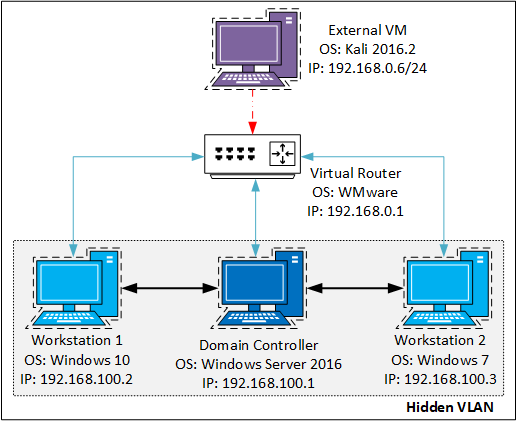
\includegraphics{NetworkDiagram.png}
\end{center}


\newpage
\noindent
\textbf{Answers:}
\begin{enumerate}
\item What is the port status if it does not allow entry or access to a service? \textbf{Closed}
\item On which port is DNS? \textbf{53}
\item What service is located on port 22? \textbf{SSH}
\item What does it mean if a ping scan has not discovered a machine? \textbf{Either the firewall is filtering the ping scan packets out before it can reach the machine, or the machine is not actually running.}
\item How can port scanning assist with identification of vulnerabilities? \textbf{May find vulnerable services running or identify promising attack vectors.}
\item The answer is \textbf{(a)}:  NMap requires one open and one closed port to perform OS identification.
   
      \item Append a -u flag before you initiate the client and server. This will tell netcat to use UDP instead of TCP.
      \item  The -l flag denotes listening , or server mode. the absence of it indicates a client mode.

NetCat originates on port 12345, yet the attacker would see the attack coming from port 54321. The piped data is a one way connection, therefore the source cannot receive any response from target. A second relay from target to source must be established to receive a response from the target computer.\end{enumerate}

\noindent
\textbf{Challenge Hints:}
\begin{enumerate}
\item In order to find all the IP addresses, scan the entire subnet. You can see which subnet you're on using \texttt{ifconfig} on a *nix box and \texttt{ipconfig} on Windows. For this tutorial, you should be scanning the same subnet that you're on.

\item Hint 1: Use -O to identify what OS is running. That might be useful information.\\
Hint 2: For this challenge start searching ports which are not common. Try to search a range of ports\\
Hint 3: Try using the -sV option to identify which services are running.\\

   \item Use the commands -l for the server to listen and on the client side use the IP address. Don't forget to add the port on which you want to listen.
   \item In order to do this challenge use the concept of the previous challenge where on the source the IP address must be present and destination must be able to listen to the port number which you assign. Remember in this challenge you will have to use the symbols " < , > " in order to specify the file name. Figure out which symbol must be present on source and which one on the destination.
\end{enumerate}

\noindent
\textbf{Changelog:}
\label{changelog}
\vspace{6mm}


\begin{tabular}{ |p{1cm}|p{3cm}|p{4cm}|p{6cm}| }
\hline
\multicolumn{4}{|c|}{Network Scanning:  NMap and NetCat} \\ \hline
\texttt{Ver.} & \texttt{Date} & \texttt{Authors} & \texttt{Changes} \\ \hline
v1 & Feb. 10th 2016 & Venkata SreeKrishna K. and Lavanya K. Galla & First draft of tutorial \\ \hline
v2 & Jun. 1st 2016 & Adam Odell & Moderate content addition and fixed grammar mistakes \\ \hline
v2.1 & Jul. 19th 2016 & Adam Odell & Added appendix and other minor enhancements \\ \hline
v4.0 & Jan. 30th 2017 & Hannah Pearson and Dillon Harris & Revised executive summary. Changed slide content and syntax, removed news slide due to time and lack of practical importance, and rearranged  NMap slides to follow a more intuitive sequence. Added Commonly Used Ports,  NMap Timing, and  NMap Firewall Evasion Options to  NMap section; removed, edited, and added questions, changing challenge 2 and tasks 1 and 3 in  NMap section; and added one question and three challenges to NetCat section  \\ \hline
v4.1 & July 8th 2017 & Ananth Jillepalli & Standardization (network layout diagram, edits, consistency, TeX markup cleaning, and more). \\ \hline
\end{tabular}


\pagebreak
% this style of bibliography shows urls
\bibliographystyle{IEEEtran}


\begin{thebibliography}{9}

\bibitem{NMap}
   \textit{NMap}. NMap Security Scanner. \\
   \url{https:// NMap.org/}

\bibitem{book}

Lyon, G.  NMap Network Scanning,
 NMap Project, The Internet, 2009.

\bibitem{nmap7}
\textit{ NMap 7 Brings Faster Scanning and Improved IPv6 Support}. 23 November 2015.\\
\url{http://www.infoworld.com/article/3007301/network-security/nmap-7-brings-faster-scanning-and-improved-ipv6-support.html}

\bibitem{rtfm}
Clark, Ben. \textit{RTFM: Red Team Field Manual}. 2013.

\bibitem{sourceforge}
\textit{SourceForge Accused of Hijacking  NMap Project Account}. 3 June 2015.\\
\burl{http://www.digitaltrends.com/computing/sourceforge-accused-of-hijacking-nmap-project-account/}

\bibitem{cookbook}

Marsh, Nicholas.  NMap Cookbook: The Fat-free Guide to Network Scanning. CreateSpace, 2010.
    
\bibitem{INmap}
\textit{Introducing  NMap}\\
\url{http://scitechconnect.elsevier.com/wp-content/uploads/2013/09/Introducing- NMap.pdf}

\bibitem{Inetcat}
\textit{Introduction to NetCat}\\
\url{http://scitechconnect.elsevier.com/wp-content/uploads/2013/09/Introduction-to-NetCat.pdf}


\bibitem{CEH}
Gregg, Michael. Certified ethical hacker (CEH) cert guide. Pearson IT Certification, 2013.



%example biblio entry
\iffalse
\bibitem{Winkler15}
    Winkler, I.
    2015
    \textit{The 'Sophisticated Attack' Myth}\\
    ComputerWorld, The Internet, 2015.
\fi 

\end{thebibliography}


\end{document}

    Contact GitHub API Training Shop Blog About 

    © 2017 GitHub, Inc. Terms Privacy Security Status Help 
